\chapter{Graficzny interfejs użytkownika}
Do stworzenia GUI (ang. Graphical User Interface) wykorzystano wcześniej wspomnianą bibliotekę PyQT5 oferującą zestaw narzędzi do budowy interfejsu użytkownika z użyciem klas QT
\section{Pierwszy etap implementacji}
Czytelny, prosty i przejrzysty interfejs użytkownika jest podstawą każdej dobrej aplikacji, niestety ze względu na wyzwania jakie niosła za sobą synchronizacja posiadanych map reprezentowanych przez zbiór plików .las z mapą geograficzną np. z Google Maps, nanoszenie zagrożeń na interaktywną mapę okazało się chwilowo poza zasięgiem.
\subsection{Mapa Tatr}
\begingroup
\begin{figure}[h]
	\centering
	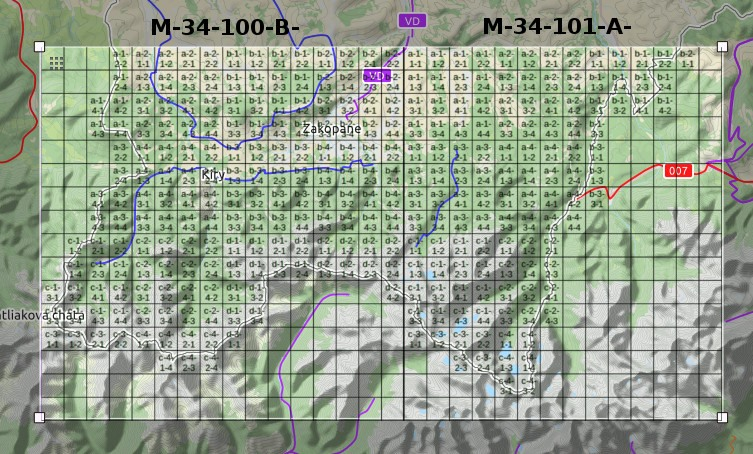
\includegraphics[scale=0.4]{tlo.png}
	\caption{Oryginalna mapa}
\end{figure}
\endgroup
\section{Etap drugi - główne okno aplikacji}
Stwierdzono, że główne okno aplikacji powinno zawierać jak najmniej zbędnych elementów i być czytelne jak i przykuwające uwagę, z tego powodu na ekranie głównym aplikacji widnieje piękny widok na Morskie Oko wraz z okalającymi je szczytami widziane ze schroniska.
\begingroup
\begin{figure}[h]
	\centering
	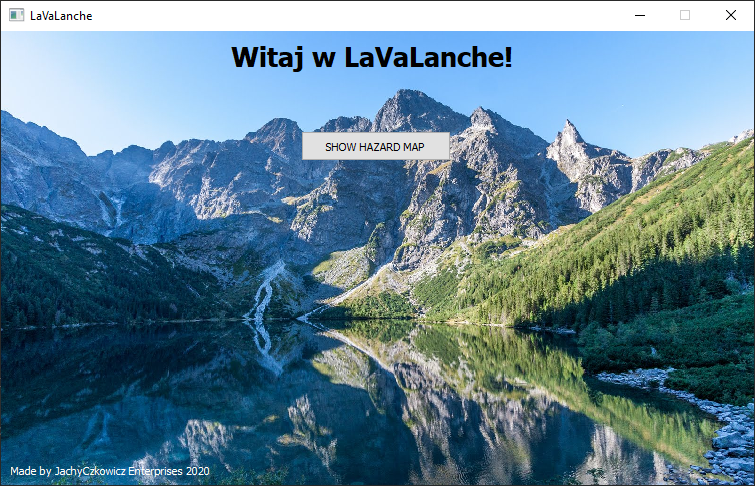
\includegraphics[scale=0.6]{main_window.png}
	\caption{Okno główne aplikacji \\ źródło: http://podrozniczeretrospekcje.blogspot.com}
\end{figure}
\endgroup

\begin{lstlisting}[language=Python,caption=Fragment pseudokodu realizującego okno główne]
	class MainWindow(QMainWindow):
		def __init__(self):
			super(MainWindow, self).__init__()
			self.setFixedSize(width, height)
			self.draw_labels()
			self.draw_buttons()
			self.set_image(path_to_image)
			self.show()
	
\end{lstlisting}

\clearpage
\section{Etap trzeci - interaktywna mapa Tatr}
Wykorzystując otrzymaną wcześniej mapę Tatr, postanowiono nałożyć na poszczególne kwadraty przyciski z których każdy odnosi się do zawartego pod nim obszaru. 

\begingroup
\begin{figure}[h]
	\centering
	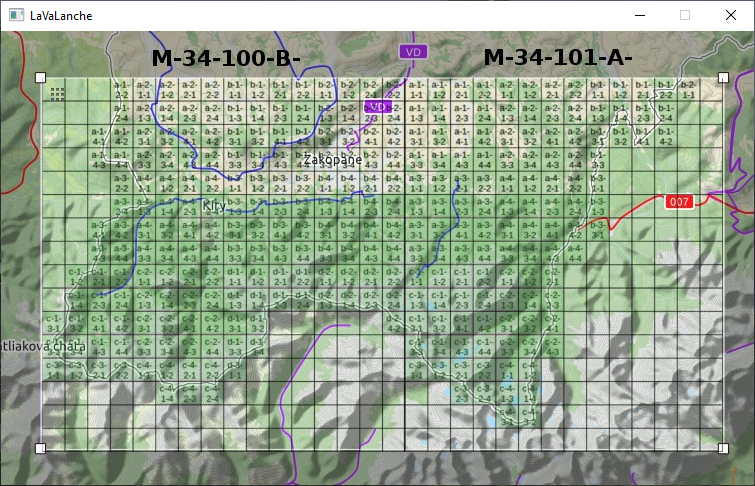
\includegraphics[scale=0.6]{map_window.png}
	\caption{Mapa z naniesionymi na nią przyciskami}
\end{figure}
\endgroup

Założono, że zagrożenie lawiną obliczane będzie tylko dla obszarów znajdujących się na południe od Zakopanego z tego względu iż ukształtowanie terenu na północ od tego miejsca praktycznie wyklucza wystąpienie jakiejkolwiek lawiny i nie ma tam historii występowania lawin, dlatego przyciski, które kolorowane są według poniższej legendy, znajdują się tylko na mniej więcej połowie obszarów. 
\begingroup
\begin{figure}[h]
	\centering
	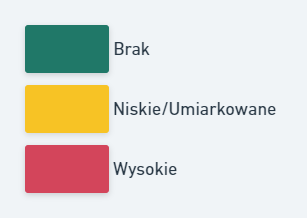
\includegraphics[scale=0.6]{kolorowanie.png}
	\caption{Legenda kolorów przycisków}
\end{figure}
\endgroup


\clearpage
\section{Etap czwarty - okna detaliczne}
Ostatni, lecz nie mniej ważny niż pozostałe etap, zakładał implementację okien detalicznych dla każdego obszaru autonomicznego tj. obszaru reprezentowanego przez jeden plik .las. W oknie detalicznym znajdują się takie dane jak:
\begin{enumerate}[label=-]
	\item stopień ryzyka
	\item charakterystyczne obiekty na danym terenie np. szczyty
	\item cechy zwiększające zagrożenie
\end{enumerate}

\begingroup
\begin{figure}[h]
	\centering
	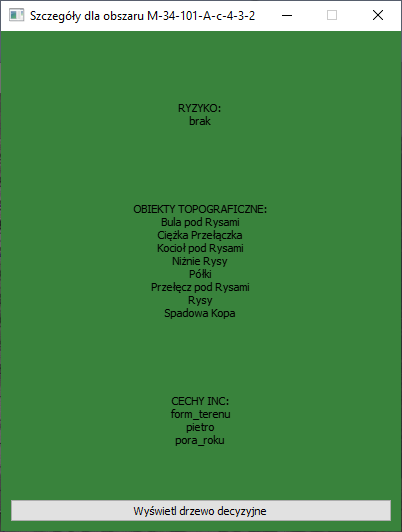
\includegraphics[scale=0.6]{detail_window.png}
	\caption{Okienko detaliczne}
\end{figure}
\endgroup
\clearpage
\section{Obsługa aplikacji i jej działanie}
Przed każdym uruchomieniem aplikacji aktualizowane są dane pogodowe z całego obszaru Tatr po polskiej stronie. Następnie ukazuje się okno główne aplikacji.

Na samym środku widnieje przycisk ''SHOW HAZARD MAP'' który po przyciśnięciu wyłącza okno główne i przechodzi do okna z interaktywną mapą obszaru.

W oknie interaktywnej mapy widnieją przyciski o kolorze odpowiadającym stopniowi zagrożnienia, każdy z przycisków włącza okno detaliczne dla odpowiedniego obszaru autonomicznego. Na chwilę obecną nie ma możliwości powrotu do ekranu głównego.








